\chapter{A Conjugal Scene}

At the Place Louis XV. the three young people separated—that is to say,
Morrel went to the Boulevards, Château-Renaud to the Pont de la
Révolution, and Debray to the Quai. Most probably Morrel and
Château-Renaud returned to their “domestic hearths,” as they say in the
gallery of the Chamber in well-turned speeches, and in the theatre of
the Rue Richelieu in well-written pieces; but it was not the case with
Debray. When he reached the wicket of the Louvre, he turned to the
left, galloped across the Carrousel, passed through the Rue Saint-Roch,
and, issuing from the Rue de la Michodière, he arrived at M. Danglars’
door just at the same time that Villefort’s landau, after having
deposited him and his wife at the Faubourg Saint-Honoré, stopped to
leave the baroness at her own house.

Debray, with the air of a man familiar with the house, entered first
into the court, threw his bridle into the hands of a footman, and
returned to the door to receive Madame Danglars, to whom he offered his
arm, to conduct her to her apartments. The gate once closed, and Debray
and the baroness alone in the court, he asked:

“What was the matter with you, Hermine? and why were you so affected at
that story, or rather fable, which the count related?”

“Because I have been in such shocking spirits all the evening, my
friend,” said the baroness.

“No, Hermine,” replied Debray; “you cannot make me believe that; on the
contrary, you were in excellent spirits when you arrived at the
count’s. M. Danglars was disagreeable, certainly, but I know how much
you care for his ill-humor. Someone has vexed you; I will allow no one
to annoy you.”

“You are deceived, Lucien, I assure you,” replied Madame Danglars; “and
what I have told you is really the case, added to the ill-humor you
remarked, but which I did not think it worth while to allude to.”

It was evident that Madame Danglars was suffering from that nervous
irritability which women frequently cannot account for even to
themselves; or that, as Debray had guessed, she had experienced some
secret agitation that she would not acknowledge to anyone. Being a man
who knew that the former of these symptoms was one of the inherent
penalties of womanhood, he did not then press his inquiries, but waited
for a more appropriate opportunity when he should again interrogate
her, or receive an avowal \textit{proprio motu}.

At the door of her apartment the baroness met Mademoiselle Cornélie,
her confidential maid.

“What is my daughter doing?” asked Madame Danglars.

“She practiced all the evening, and then went to bed,” replied
Mademoiselle Cornélie.

“Yet I think I hear her piano.”

“It is Mademoiselle Louise d’Armilly, who is playing while Mademoiselle
Danglars is in bed.”

“Well,” said Madame Danglars, “come and undress me.”

They entered the bedroom. Debray stretched himself upon a large couch,
and Madame Danglars passed into her dressing-room with Mademoiselle
Cornélie.

“My dear M. Lucien,” said Madame Danglars through the door, “you are
always complaining that Eugénie will not address a word to you.”

“Madame,” said Lucien, playing with a little dog, who, recognizing him
as a friend of the house, expected to be caressed, “I am not the only
one who makes similar complaints, I think I heard Morcerf say that he
could not extract a word from his betrothed.”

“True,” said Madame Danglars; “yet I think this will all pass off, and
that you will one day see her enter your study.”

“My study?”

“At least that of the minister.”

“Why so!”

“To ask for an engagement at the Opera. Really, I never saw such an
infatuation for music; it is quite ridiculous for a young lady of
fashion.”

Debray smiled. “Well,” said he, “let her come, with your consent and
that of the baron, and we will try and give her an engagement, though
we are very poor to pay such talent as hers.”

“Go, Cornélie,” said Madame Danglars, “I do not require you any
longer.”

Cornélie obeyed, and the next minute Madame Danglars left her room in a
charming loose dress, and came and sat down close to Debray. Then she
began thoughtfully to caress the little spaniel. Lucien looked at her
for a moment in silence.

“Come, Hermine,” he said, after a short time, “answer
candidly,—something vexes you—is it not so?”

\begin{figure}[ht]
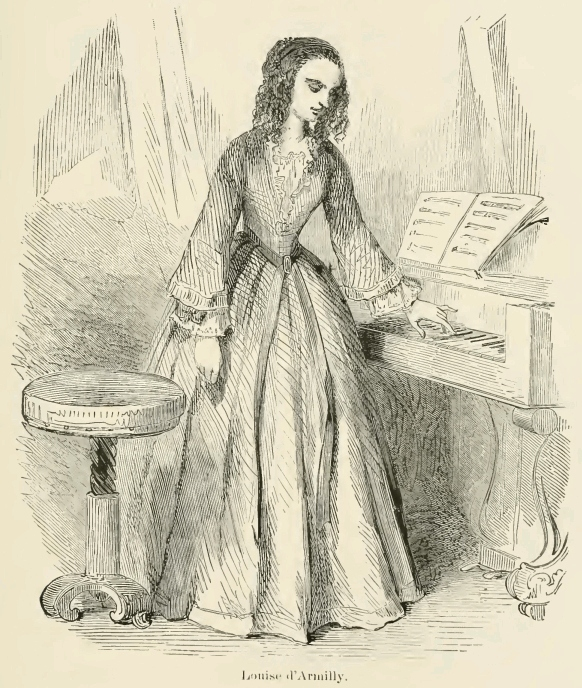
\includegraphics[width=\textwidth]{30239m.jpg}
\end{figure}

“Nothing,” answered the baroness.

And yet, as she could scarcely breathe, she rose and went towards a
looking-glass. “I am frightful tonight,” she said. Debray rose,
smiling, and was about to contradict the baroness upon this latter
point, when the door opened suddenly. M. Danglars appeared; Debray
reseated himself. At the noise of the door Madame Danglars turned
round, and looked upon her husband with an astonishment she took no
trouble to conceal.

“Good-evening, madame,” said the banker; “good-evening, M. Debray.”

Probably the baroness thought this unexpected visit signified a desire
to make up for the sharp words he had uttered during the day. Assuming
a dignified air, she turned round to Debray, without answering her
husband.

“Read me something, M. Debray,” she said. Debray, who was slightly
disturbed at this visit, recovered himself when he saw the calmness of
the baroness, and took up a book marked by a mother-of-pearl knife
inlaid with gold.

“Excuse me,” said the banker, “but you will tire yourself, baroness, by
such late hours, and M. Debray lives some distance from here.”

Debray was petrified, not only to hear Danglars speak so calmly and
politely, but because it was apparent that beneath outward politeness
there really lurked a determined spirit of opposition to anything his
wife might wish to do. The baroness was also surprised, and showed her
astonishment by a look which would doubtless have had some effect upon
her husband if he had not been intently occupied with the paper, where
he was looking to see the closing stock quotations. The result was,
that the proud look entirely failed of its purpose.

“M. Lucien,” said the baroness, “I assure you I have no desire to
sleep, and that I have a thousand things to tell you this evening,
which you must listen to, even though you slept while hearing me.”

“I am at your service, madame,” replied Lucien coldly.

“My dear M. Debray,” said the banker, “do not kill yourself tonight
listening to the follies of Madame Danglars, for you can hear them as
well tomorrow; but I claim tonight and will devote it, if you will
allow me, to talk over some serious matters with my wife.”

This time the blow was so well aimed, and hit so directly, that Lucien
and the baroness were staggered, and they interrogated each other with
their eyes, as if to seek help against this aggression, but the
irresistible will of the master of the house prevailed, and the husband
was victorious.

“Do not think I wish to turn you out, my dear Debray,” continued
Danglars; “oh, no, not at all. An unexpected occurrence forces me to
ask my wife to have a little conversation with me; it is so rarely I
make such a request, I am sure you cannot grudge it to me.”

Debray muttered something, bowed and went out, knocking himself against
the edge of the door, like Nathan in \textit{Athalie}.

“It is extraordinary,” he said, when the door was closed behind him,
“how easily these husbands, whom we ridicule, gain an advantage over
us.”

\begin{figure}[ht]
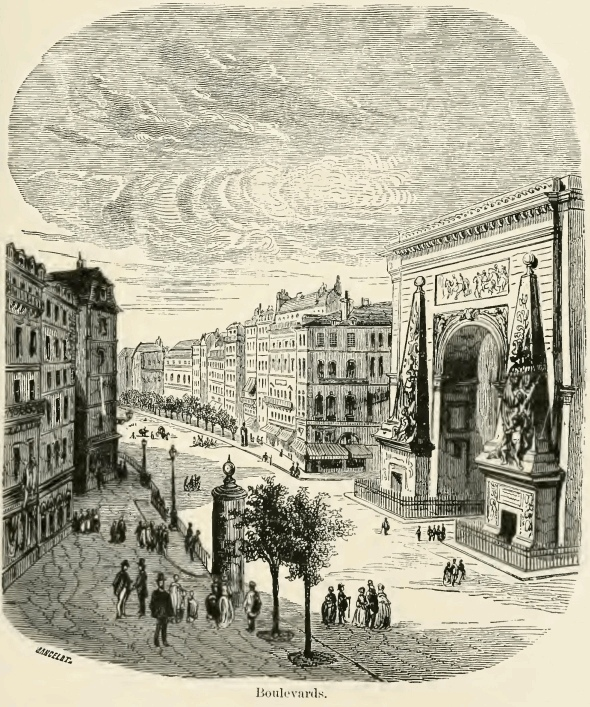
\includegraphics[width=\textwidth]{30241m.jpg}
\end{figure}

Lucien having left, Danglars took his place on the sofa, closed the
open book, and placing himself in a dreadfully dictatorial attitude, he
began playing with the dog; but the animal, not liking him as well as
Debray, and attempting to bite him, Danglars seized him by the skin of
his neck and threw him upon a couch on the other side of the room. The
animal uttered a cry during the transit, but, arrived at its
destination, it crouched behind the cushions, and stupefied at such
unusual treatment remained silent and motionless.

“Do you know, sir,” asked the baroness, “that you are improving?
Generally you are only rude, but tonight you are brutal.”

“It is because I am in a worse humor than usual,” replied Danglars.
Hermine looked at the banker with supreme disdain. These glances
frequently exasperated the pride of Danglars, but this evening he took
no notice of them.

“And what have I to do with your ill-humor?” said the baroness,
irritated at the impassibility of her husband; “do these things concern
me? Keep your ill-humor at home in your money boxes, or, since you have
clerks whom you pay, vent it upon them.”

“Not so,” replied Danglars; “your advice is wrong, so I shall not
follow it. My money boxes are my Pactolus, as, I think, M. Demoustier
says, and I will not retard its course, or disturb its calm. My clerks
are honest men, who earn my fortune, whom I pay much below their
deserts, if I may value them according to what they bring in; therefore
I shall not get into a passion with them; those with whom I will be in
a passion are those who eat my dinners, mount my horses, and exhaust my
fortune.”

“And pray who are the persons who exhaust your fortune? Explain
yourself more clearly, I beg, sir.”

“Oh, make yourself easy!—I am not speaking riddles, and you will soon
know what I mean. The people who exhaust my fortune are those who draw
out 700,000 francs in the course of an hour.”

“I do not understand you, sir,” said the baroness, trying to disguise
the agitation of her voice and the flush of her face.

“You understand me perfectly, on the contrary,” said Danglars: “but, if
you will persist, I will tell you that I have just lost 700,000 francs
upon the Spanish loan.”

“And pray,” asked the baroness, “am I responsible for this loss?”

“Why not?”

“Is it my fault you have lost 700,000 francs?”

“Certainly it is not mine.”

“Once for all, sir,” replied the baroness sharply, “I tell you I will
not hear cash named; it is a style of language I never heard in the
house of my parents or in that of my first husband.”

“Oh, I can well believe that, for neither of them was worth a penny.”

“The better reason for my not being conversant with the slang of the
bank, which is here dinning in my ears from morning to night; that
noise of jingling crowns, which are constantly being counted and
re-counted, is odious to me. I only know one thing I dislike more,
which is the sound of your voice.”

“Really?” said Danglars. “Well, this surprises me, for I thought you
took the liveliest interest in all my affairs!”

\begin{figure}[ht]
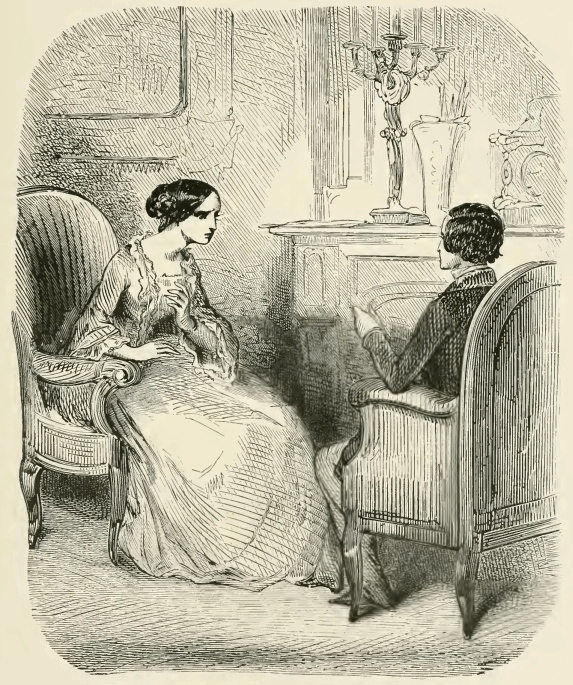
\includegraphics[width=\textwidth]{30243m.jpg}
\end{figure}

“I? What could put such an idea into your head?”

“Yourself.”

“Ah?—what next?”

“Most assuredly.”

“I should like to know upon what occasion?”

“Oh, \textit{mon Dieu!} that is very easily done. Last February you were the
first who told me of the Haitian funds. You had dreamed that a ship had
entered the harbor at Le Havre, that this ship brought news that a
payment we had looked upon as lost was going to be made. I know how
clear-sighted your dreams are; I therefore purchased immediately as
many shares as I could of the Haitian debt, and I gained 400,000 francs
by it, of which 100,000 have been honestly paid to you. You spent it as
you pleased; that was your business. In March there was a question
about a grant to a railway. Three companies presented themselves, each
offering equal securities. You told me that your instinct,—and although
you pretend to know nothing about speculations, I think on the
contrary, that your comprehension is very clear upon certain
affairs,—well, you told me that your instinct led you to believe the
grant would be given to the company called the Southern. I bought two
thirds of the shares of that company; as you had foreseen, the shares
trebled in value, and I picked up a million, from which 250,000 francs
were paid to you for pin-money. How have you spent this 250,000
francs?—it is no business of mine.”

“When are you coming to the point?” cried the baroness, shivering with
anger and impatience.

“Patience, madame, I am coming to it.”

“That’s fortunate.”

“In April you went to dine at the minister’s. You heard a private
conversation respecting Spanish affairs—on the expulsion of Don Carlos.
I bought some Spanish shares. The expulsion took place and I pocketed
600,000 francs the day Charles V. repassed the Bidassoa. Of these
600,000 francs you took 50,000 crowns. They were yours, you disposed of
them according to your fancy, and I asked no questions; but it is not
the less true that you have this year received 500,000 livres.”

“Well, sir, and what then?”

“Ah, yes, it was just after this that you spoiled everything.”

“Really, your manner of speaking——”

“It expresses my meaning, and that is all I want. Well, three days
after that you talked politics with M. Debray, and you fancied from his
words that Don Carlos had returned to Spain. Well, I sold my shares,
the news got out, and I no longer sold—I gave them away, next day I
find the news was false, and by this false report I have lost 700,000
francs.”

“Well?”

“Well, since I gave you a fourth of my gains, I think you owe me a
fourth of my losses; the fourth of 700,000 francs is 175,000 francs.”

“What you say is absurd, and I cannot see why M. Debray’s name is mixed
up in this affair.”

“Because if you do not possess the 175,000 francs I reclaim, you must
have lent them to your friends, and M. Debray is one of your friends.”

\begin{figure}[ht]
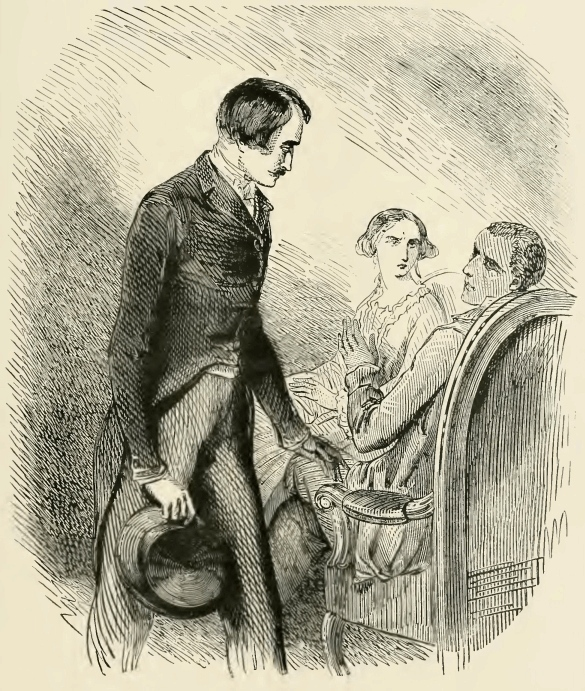
\includegraphics[width=\textwidth]{30245m.jpg}
\end{figure}

“For shame!” exclaimed the baroness.

“Oh, let us have no gestures, no screams, no modern drama, or you will
oblige me to tell you that I see Debray leave here, pocketing the whole
of the 500,000 livres you have handed over to him this year, while he
smiles to himself, saying that he has found what the most skilful
players have never discovered—that is, a roulette where he wins without
playing, and is no loser when he loses.”

The baroness became enraged.

“Wretch!” she cried, “will you dare to tell me you did not know what
you now reproach me with?”

“I do not say that I did know it, and I do not say that I did not know
it. I merely tell you to look into my conduct during the last four
years that we have ceased to be husband and wife, and see whether it
has not always been consistent. Some time after our rupture, you wished
to study music, under the celebrated baritone who made such a
successful appearance at the Théâtre Italien; at the same time I felt
inclined to learn dancing of the \textit{danseuse} who acquired such a
reputation in London. This cost me, on your account and mine, 100,000
francs. I said nothing, for we must have peace in the house; and
100,000 francs for a lady and gentleman to be properly instructed in
music and dancing are not too much. Well, you soon become tired of
singing, and you take a fancy to study diplomacy with the minister’s
secretary. You understand, it signifies nothing to me so long as you
pay for your lessons out of your own cash box. But today I find you are
drawing on mine, and that your apprenticeship may cost me 700,000
francs per month. Stop there, madame, for this cannot last. Either the
diplomatist must give his lessons gratis, and I will tolerate him, or
he must never set his foot again in my house;—do you understand,
madame?”

“Oh, this is too much,” cried Hermine, choking, “you are worse than
despicable.”

“But,” continued Danglars, “I find you did not even pause there——”

“Insults!”

“You are right; let us leave these facts alone, and reason coolly. I
have never interfered in your affairs excepting for your good; treat me
in the same way. You say you have nothing to do with my cash box. Be it
so. Do as you like with your own, but do not fill or empty mine.
Besides, how do I know that this was not a political trick, that the
minister enraged at seeing me in the opposition, and jealous of the
popular sympathy I excite, has not concerted with M. Debray to ruin
me?”

“A probable thing!”

“Why not? Who ever heard of such an occurrence as this?—a false
telegraphic despatch—it is almost impossible for wrong signals to be
made as they were in the last two telegrams. It was done on purpose for
me—I am sure of it.”

“Sir,” said the baroness humbly, “are you not aware that the man
employed there was dismissed, that they talked of going to law with
him, that orders were issued to arrest him and that this order would
have been put into execution if he had not escaped by flight, which
proves that he was either mad or guilty? It was a mistake.”

“Yes, which made fools laugh, which caused the minister to have a
sleepless night, which has caused the minister’s secretaries to blacken
several sheets of paper, but which has cost me 700,000 francs.”

“But, sir,” said Hermine suddenly, “if all this is, as you say, caused
by M. Debray, why, instead of going direct to him, do you come and tell
me of it? Why, to accuse the man, do you address the woman?”

“Do I know M. Debray?—do I wish to know him?—do I wish to know that he
gives advice?—do I wish to follow it?—do I speculate? No; you do all
this, not I.”

“Still it seems to me, that as you profit by it——”

Danglars shrugged his shoulders. “Foolish creature,” he exclaimed.
“Women fancy they have talent because they have managed two or three
intrigues without being the talk of Paris! But know that if you had
even hidden your irregularities from your husband, who has but the
commencement of the art—for generally husbands \textit{will} not see—you would
then have been but a faint imitation of most of your friends among the
women of the world. But it has not been so with me,—I see, and always
have seen, during the last sixteen years. You may, perhaps, have hidden
a thought; but not a step, not an action, not a fault, has escaped me,
while you flattered yourself upon your address, and firmly believed you
had deceived me. What has been the result?—that, thanks to my pretended
ignorance, there is none of your friends, from M. de Villefort to M.
Debray, who has not trembled before me. There is not one who has not
treated me as the master of the house,—the only title I desire with
respect to you; there is not one, in fact, who would have dared to
speak of me as I have spoken of them this day. I will allow you to make
me hateful, but I will prevent your rendering me ridiculous, and, above
all, I forbid you to ruin me.”

The baroness had been tolerably composed until the name of Villefort
had been pronounced; but then she became pale, and, rising, as if
touched by a spring, she stretched out her hands as though conjuring an
apparition; she then took two or three steps towards her husband, as
though to tear the secret from him, of which he was ignorant, or which
he withheld from some odious calculation,—odious, as all his
calculations were.

“M. de Villefort!—What do you mean?”

“I mean that M. de Nargonne, your first husband, being neither a
philosopher nor a banker, or perhaps being both, and seeing there was
nothing to be got out of a king’s attorney, died of grief or anger at
finding, after an absence of nine months, that you had been \textit{enceinte}
six. I am brutal,—I not only allow it, but boast of it; it is one of
the reasons of my success in commercial business. Why did he kill
himself instead of you? Because he had no cash to save. My life belongs
to my cash. M. Debray has made me lose 700,000 francs; let him bear his
share of the loss, and we will go on as before; if not, let him become
bankrupt for the 250,000 livres, and do as all bankrupts do—disappear.
He is a charming fellow, I allow, when his news is correct; but when it
is not, there are fifty others in the world who would do better than
he.”

Madame Danglars was rooted to the spot; she made a violent effort to
reply to this last attack, but she fell upon a chair thinking of
Villefort, of the dinner scene, of the strange series of misfortunes
which had taken place in her house during the last few days, and
changed the usual calm of her establishment to a scene of scandalous
debate.

Danglars did not even look at her, though she did her best to faint. He
shut the bedroom door after him, without adding another word, and
returned to his apartments; and when Madame Danglars recovered from her
half-fainting condition, she could almost believe that she had had a
disagreeable dream.
